\documentclass[10pt]{article}
\usepackage[left=0.9in,top=0.9in,bottom=0.9in,right=0.9in]{geometry}
\usepackage{setspace}
\usepackage{titlesec}
\usepackage{graphicx}
\usepackage{float}
\usepackage{mathtools}
\usepackage{amsmath}
\usepackage[font=small,labelfont=bf,labelsep=period]{caption}
\usepackage[english]{babel}
\usepackage{indentfirst}
\usepackage{array}
\usepackage{makecell}
\usepackage[usenames,dvipsnames]{xcolor}
\usepackage{multirow}
\usepackage{tabularx}
\usepackage{arydshln}
\usepackage{caption}
\usepackage{subcaption}
\usepackage{xfrac}
\usepackage[numbers,sort&compress]{natbib}
\usepackage{enumitem}
\usepackage{lipsum}
\usepackage{hyperref}
\usepackage{caption}
\usepackage{amssymb}
\setlength{\bibsep}{0pt}

\usepackage{listings}
\lstset{
  language=Python,
  aboveskip=3mm,
  belowskip=3mm,
  showstringspaces=false,
  columns=flexible,
  basicstyle={\small\ttfamily},
  breaklines=true,
  breakatwhitespace=true,
  tabsize=3,
  numbers=none,
  xleftmargin=0em,
  framexleftmargin=3.5em
}

%\usepackage{setspace}
%\onehalfspacing
\linespread{1.3}  % one-half spacing

%\pagestyle{fancy} 
%\fancyhead[LE,RO]{\today}
%\fancyhead[C]{NE 255}
%\fancyhead[LO,RE]{D. Hellfeld}
%\fancyfoot[C]{\thepage\ of \pageref{LastPage}}
%\renewcommand{\headrulewidth}{0.4pt}
%\renewcommand{\footrulewidth}{0.4pt}

%\pagestyle{empty}

% Set up figure/table captions
\addto\captionsenglish{\renewcommand{\figurename}{Fig.}}
\addto\captionsenglish{\renewcommand{\tablename}{\small Table}}
\renewcommand{\thetable}{\Roman{table}}
\captionsetup[table]{labelfont = normal, labelsep=period, singlelinecheck=false}
\captionsetup[figure]{labelfont=normal, labelsep=period, singlelinecheck=true}

%\setlength\parindent{0pt}

% Set up section\subsection title formats
\renewcommand{\thesection}{\Roman{section}}
\renewcommand{\thesubsection}{\thesection.\Roman{subsection}}
\titleformat*{\section}{\normalsize\bfseries}
\titleformat*{\subsection}{\normalsize\bfseries}

\begin{document}

\begin{centering}
\textbf{Monte Carlo Simulation and Analysis Framework for a CdZnTe-based Spherical Coded\\[-5pt] Aperture and Compton Gamma-ray Imager}\\
\vspace{5pt}
\emph{Interim Report}\\
\vspace{5pt}
NE 255 - Numerical Simulation in Radiation Transport \\[-5pt]
University of California, Berkeley \\[-5pt]
Department of Nuclear Engineering\\
\vspace{5pt}
Daniel Hellfeld\\
\vspace{5pt}
November 15, 2016 \\
\end{centering}


% -----------------------------------------------------------------------
\section{Introduction}

The goal of this project is to improve a Geant4 \cite{Agostinelli2003} Monte Carlo simulation for the Portable Radiation Imaging Spectroscopy and Mapping (PRISM) detector system under development at Lawrence Berkeley National Laboratory (LBNL) (see \hyperlink{fig1}{Fig.\,1a-b}) and to develop a small suite of analysis tools. The PRISM system consists of cm$^3$ CdZnTe (CZT) coplanar grid (CPG) gamma-ray detectors arranged on the inner surface of a 14 cm diameter sphere. There are 192 available detector locations on the sphere, and an active coded arrangement, or a pattern of occupied and empty locations (see \hyperlink{fig1}{Fig.\,1c}), of the detectors allows for gamma-ray imaging in 4$\pi$ using both coded aperture (low energy) and Compton imaging (high energy) modalities. The purpose of the simulation is to determine the response of the system to radioactive sources of varying energies, intensities, and spatial distributions in the entire 4$\pi$ field-of-view (FOV). The simulated response can then be used as a tool to inform prototype design, for characterization, and for image reconstruction. 

The original simulation was developed in order to generate a simple approximation of the coded aperture response in the far-field limit (parallel rays at infinity). The simulation essentially functioned as a ray-tracer (i.e. no scattering, no secondary electron tracking), however some physics was included to account for the depth-of-interaction (DOI) in each detector (which is used to significantly improve the coded aperture reconstruction). This project aims to restructure and upgrade the original simulation to include more functionality such as scattering physics, secondary electron production and tracking, multi-site events, geometry modification, and near-field sources with varying strengths and distributions. In addition to the simulation, analysis tools used for event sequencing, data preprocessing, and 2D/3D image reconstruction will be developed. The ultimate objective of this project is to develop a high-fidelity, robust, flexible, well-documented, and easy to use simulation and analysis framework that can be used to answer a variety of research questions for the novel concept of a spherical coded aperture and Compton imaging system. 

This report will first discuss the mathematics and algorithms used in the simulation and analysis framework - including derivations of the Monte Carlo sampling functions and image reconstruction methods for both coded aperture and Compton imaging modalities. Next, an overview of the developed code will be presented, outlining how to run the simulation and analysis scripts. Simple example inputs will be included, as well as output results. The methods of verification and validation will then be addressed, including the input and output of test cases used in development. Finally, the work will be summarized and future work will be outlined. 

\begin{figure}[htb]
\hypertarget{fig1}{}
\centering
\begin{tabular}{ccc}
	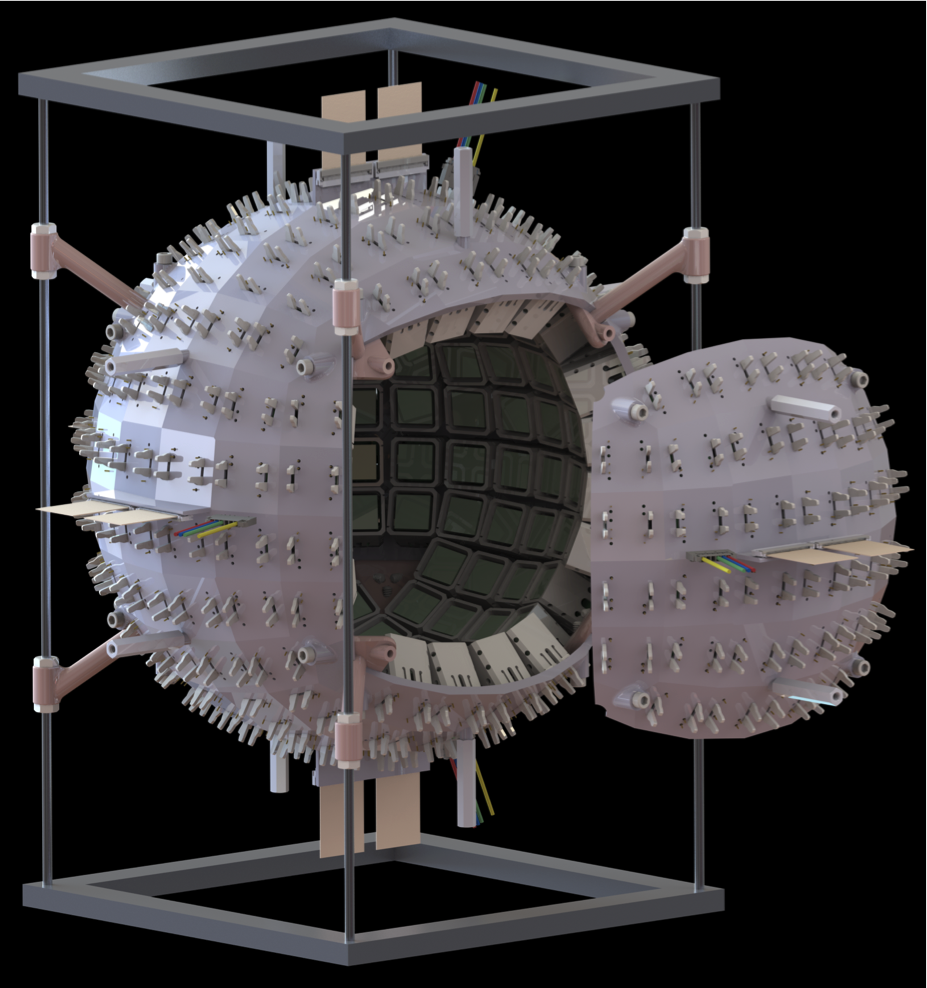
\includegraphics[height=130pt]{Figures/PRISM_Design.png} & 
	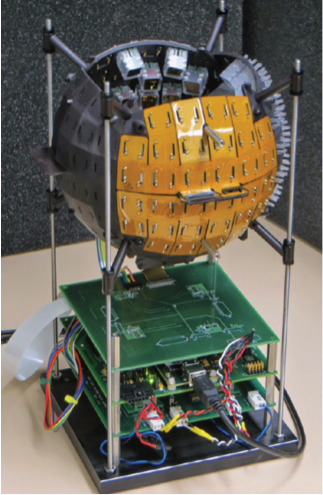
\includegraphics[height=130pt]{Figures/PRISM_Prototype.png} & 
	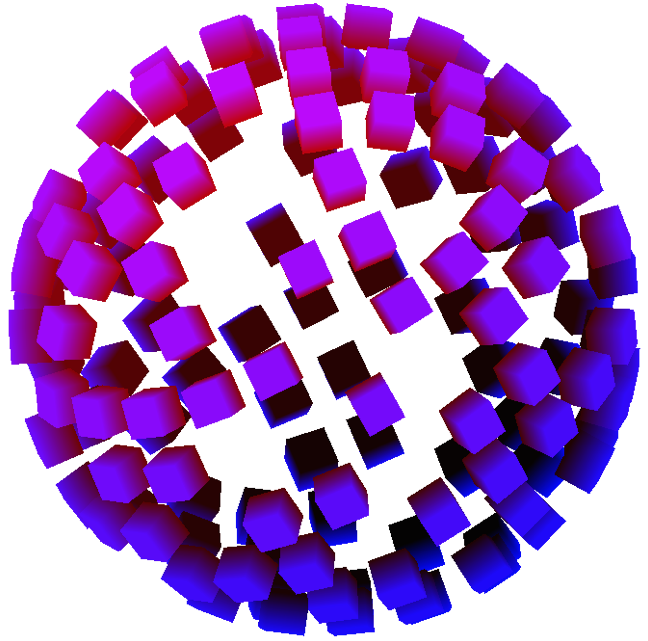
\includegraphics[height=130pt]{Figures/Masked_Configuration.png} \\
	\scriptsize{(a)} & \scriptsize{(b)} & \scriptsize{(c)} \\[-6pt]
\end{tabular}
\caption{(a) Modular design of PRISM. (b) PRISM prototype system currently under development at LBNL. (c) Example coded arrangement of detectors.}
\end{figure}






% -----------------------------------------------------------------------
\section{Mathematics}

A simple handheld radiation detector (such as a simple NaI scintillation crystal attached to a photomultiplier tube) can be used to map radiation. The count rate is recorded while the system is moved through space, and an intensity map can be produced in 3D. This method, however, is not optimal because of the low efficiency (only one detector), the poor spatial resolution, and the dependence on the users path and proximity to the source. To produce a freely moving handheld system with high efficiency and high energy/spatial resolution, a move clever approach is needed. Coded aperture is a technique first developed for X-ray astronomy and uses the principle of unique photon modulation for image reconstruction \cite{FenimoreCannon1978}. Typically an array of position sensitive photon detectors are placed behind an array of photon absorbing material (such as lead or tungsten) such that the detection pattern in the detector array is unique to a location in the image space. In the case of PRISM, there is no lead or tungsten to avoid weight and instead more detectors are used. At low energies, the CZT easily attenuates the photons and acts a mask (the counts in the mask detectors can also be rejected). Moreover, using detectors instead of a passive mask increases the detection efficiency.

To reconstruct the image, the absorbing array (typically referred to as the \emph{mask} or the \emph{aperture}) is used to deconvolve the detected image (which by itself will not reveal anything about the source location). Typically this is represented by the following:
%
\begin{equation}
	P = A \ast O + N\,,
\end{equation}

\noindent where $P$ is the detected image, $A$ is the aperture, $O$ is the source object, $N$ is noise, and $\ast$ represents the convolution operator. In one dimension this is given by
%
\begin{equation}
	f(x) \ast g(x) = \int_{-\infty}^\infty du f(u)g(x-u)\,.
\end{equation}

\noindent To solve for the source object $O$, the convolution theorem
%
\begin{equation}
	\mathfrak{F}(f(x) \ast g(x)) = \mathfrak{F}(f(x)) \mathfrak{F}(g(x)) = F(k)G(k)\,,
\end{equation}

\noindent is used, where $\mathfrak{F}$ is the Fourier transform operator and $k$ is spatial frequency. In doing so results in
%
\begin{align}
	%\mathfrak{F}(P) = \mathfrak{F}(A) \mathfrak{F}(O) + \mathfrak{F}(N)\,, \\
	\mathfrak{F}(O) = \frac{\mathfrak{F}(P)}{\mathfrak{F}(A)} + \frac{\mathfrak{F}(N)}{\mathfrak{F}(A)}\,,  \\
	\hat{O} = \mathfrak{F}^{-1}\left(\frac{\mathfrak{F}(P)}{\mathfrak{F}(A)} + \frac{\mathfrak{F}(N)}{\mathfrak{F}(A)}\right)\,, \\
	\hat{O} = O + \mathfrak{F}^{-1}\left( \frac{\mathfrak{F}(N)}{\mathfrak{F}(A)}\right)\,.
\end{align}

\noindent This method of deconvolution is simple and straightforward, however since the aperture is an array of ones and zeros, the $\mathfrak{F}(A)$ term can be small. This results is a large noise gain, rendering the deconvolution image useless. Several techniques can be used to work around this problem, typically using specific mask patterns or, more importantly, by using a different reconstruction technique. Several methods exist, but the three most frequently used are back-projection, cross correlation and maximum likelihood expectation maximization (MLEM) \cite{LangeCarson1984}. This report will focus solely on MLEM. The derivation of the MLEM method is as follows. Assume the measured detector counts are Poisson distributed, such that the probability of observing a count $k$ in detector $\lambda$ is 
%
\begin{equation}
	P(z=k)  = \frac{e^{-\lambda} \lambda^k}{k!}\,,
\end{equation}

\noindent and thus the likelihood over all detector bins and image pixels is 
%
\begin{equation}
	L(X,\lambda) = \prod_{i,j\in I_i} \ \frac{e^{-C_{ij}\lambda_j} (C_{ij}\lambda)^{X_{ij}}}{X_{ij}!}\,,
\end{equation}

\noindent where $i$ is the detector index, $j$ is the image pixel index, $I_i$ are the set of image pixels that contribute to detector $i$, $C_{ij}$ is the probability of getting a count in detector $i$ from source $j$ (system response), $\lambda_j$ is the intensity at image pixel $j$, and $X_{ij}$ is the number of photons emitted from source $j$ to detector $i$. Also note that the total number of counts in detector $i$ is given by $Y_i=\sum_{j \in I_i} X_{ij}$. To make this more manageable, the log-likelihood function is used
%
\begin{equation}
	\log L(X,\lambda) = \sum_i \sum_{j \in I_i} \left[ -C_{ij} \lambda_j + X_{ij} \log (C_{ij} \lambda) - \log (X_{ij}!) \right]\,.
\end{equation}

\noindent The conditional expectation of the log-likelihood is taken with respect to $Y$ and the current source distribution $\lambda^n$
%
\begin{equation}
	E[\log L(X,\lambda) | Y,\lambda^n] = \sum_i \sum_{j \in I_i} \left[   -C_{ij} \lambda_j + \frac{C_{ij}\lambda_j^n Y_i}{\sum_{k \in I_i}C_{ij}\lambda_k^n }   \log (C_{ij} \lambda)   \right]\,.
\end{equation}

\noindent The expectation is then maximized, by taking a partial derivative with respect to $\lambda_j$ and setting it equal to 0
 %
 \begin{equation}
	\frac{\partial}{\partial \lambda_j} E[\log L(X,\lambda) | Y,\lambda^n] = 0\,.
\end{equation}

\noindent Solving the above, the final result is concise and gives a relation between the current source distribution and the next iteration
%
 \begin{equation}
	\lambda_j^{n+1} = \frac{\lambda_j^n}{\sum\limits_{i \in J_j}C_{ij}} \sum_{i \in J_j} \frac{C_{ij}Y_i}{\sum\limits_{k \in I_i}C_{ik}\lambda_k^n}\,,
\end{equation}

\noindent where $J_j$ is the set of detectors to which image pixel $j$ contributes. This results provides an iterative method to reconstruct the source distribution without the noise gain effects inherent in deconvolution. \textbf{Include note on convergence criteria here}. It is now clear that the simulation is needed to generate the system response ($C_{ij}$) in order to perform image reconstruction. Due to the iterative nature of this method, it is inherently slower than deconvolution. In most cases the technique can be easily vectorized and computed quickly, however it can become difficult when attempting to reconstruct in a list-mode fashion (count by count) in real time.

Coded aperture imaging is powerful when the photon energy is low, because the modulation (or mechanical collimation) is what produces the unique coding on the detected image. If the energy becomes too large, the attenuation decreases and the photons can penetrate the mask. With higher energy photons, an electric collimation technique such as Compton imaging can be used. Gamma-rays can scatter in the detectors and eventually be stopped via photoelectric absorption. By measuring the interaction positions and energy depositions of the individual interactions, the photon path can be tracked through the system. The first two interactions can then be used to determine a cone of incident angles from which the incident photon originated from. The image is reconstructed by the overlap of multiple cones (in 3D) or circles (in 2D). \textbf{Mathematics of Compton scattering, event sequencing, and cone backprojection goes here}. \textbf{Also need to include citations for Compton imaging.}

The mathematics involved in Monte Carlo transport of photons in the detector system is quite simple. There are three main computations occurring in the simulation - sampling the distance into a material in which an interaction takes (\emph{next collision distance}), sampling the interaction process, and if a scattering event, sampling the energy and angle of the scattered photon. At this point the physics of electron transport will be neglected. First, sampling the distance to interaction is done essentially by inverting the probability density function (PDF). The probability of not having an interaction (any interaction) after a distance $x$, and then having an interaction at $x$ is given by 
%
 \begin{equation}
	p(x) = \Sigma_t e^{-\Sigma_t x}\,, \quad x \geq 0\,,
\end{equation}

\noindent where $\Sigma_t$ is the total macroscopic cross-section of the interaction. The PDF is integrated up to a distance $x$ and set equal to a random number, $\xi$, between 0 and 1
%
 \begin{align}
	\xi = P(x) &= \int_0^x \Sigma_t e^{-\Sigma_t s} ds \,, \\
	&= 1-e^{-\Sigma_t x} \,.
\end{align}

\noindent Now solve for $x$ noting that $1-\xi$ is also a random number which is just replaced by $\xi$
%
 \begin{align}
	x = \frac{-\log(\xi)}{\Sigma_t} \,.
\end{align}

\noindent This is calculated at every step in the particle track and compared to the distance to the next boundary in the geometry. If the next collision distance is larger than the distance to the boundary, the particle is moved to the boundary and the next collision distance is resampled in the new material. Once an interaction has occurred, the type of interaction is determined by first determining the probability of each interaction occurring. If, for example, three cross-sections exist, the probability of the three occurring are given by  
%
\begin{align}
	p(\sigma_1) = \frac{\sigma_1}{\sigma_1 + \sigma_2 + \sigma_3} \\
	p(\sigma_2) = \frac{\sigma_2}{\sigma_1 + \sigma_2 + \sigma_3} \\
	p(\sigma_3) = \frac{\sigma_3}{\sigma_1 + \sigma_2 + \sigma_3}
\end{align}

\noindent where $\sigma$ is the microscopic cross-section and $p(\sigma_1) + p(\sigma_2) + p(\sigma_3) = 1$. Using the probabilities, a random number between 0 and 1 can be generated and a section of the domain can be designated for each interaction, where the size of the domain is proportional to the probability of it occurring. Finally, if the interaction is a scattering interaction, the energy and direction of the scattered photon must be sampled. If the scattering is a Rayleigh scattering, the energy is unchanged, but the outgoing direction may be different than the incoming direction. The outgoing direction can be sampled by performing the technique above but now using the Rayleigh scattering differential cross-section as the PDF. \textbf{Show the cross-section here}. If the interaction is Compton scattering, the outgoing direction is sampled from the differential cross-section as well, also known as the Klein-Nishina formula. \textbf{Show the cross section here}. Once the outgoing direction is sampled, the outgoing energy can be calculated analytically using the Compton scattering equation. \textbf{Show the scattering equation here}. 






% -----------------------------------------------------------------------
\section{Algorithms}

The simulation is built around the Monte Carlo toolkit, Geant4. At the heart of Geant4 lies a simple Monte Carlo algorithm for transporting particles. Individual particles, as well as any secondary particles produced, are tracked from birth to death given some initial conditions and underlying physics. This is accomplished by using the sampling techniques discussed above. The geometry is built first, detailing the size, position, and material of the objects in the system. A particle is then given to the tracker with a particle type, energy, position, momentum direction, and relevant physics. Each step in the particle track is then determined by randomly sampling the next collision distance and comparing to the next boundary distance. The particle is moved accordingly and the interaction is then randomly sampled (including the interaction type, the outgoing energy and direction, and the production of any secondary particles). If any secondary particles are produced due to an interaction, the primary particle track is paused while the secondary particle tracks are followed to completion one by one. At each step in the track, relevant information is stored in memory. This can include position, energy, time, event number, track number, current volume, original source location, etc. This process continues until the particle is killed (e.g.~absorbed) or leaves the system of interest. Once the particle track is completed, the next particle is given to the tracker and the process is repeated. Following the termination of the last particle sent to the tracker, the stored information for all particles is written to an output file of some kind (text, binary, ROOT, etc.). For the system response generation, many particles are simulated for each source location. Particles are simulated at each source location sequentially. A simple overview of this algorithm is given as follows

\begin{lstlisting}
Define geometry
Define physics
For each source location:
	For each incident particle:
		Define type, energy, position, and  direction
		While still in the system:
			Sample next collision distance
			Compare to next boundary distance, move accordingly
			Sample interaction
			Sample outgoing information and secondary particles
			Store relevant information
			Track any secondary particles emitted
	Dump stored information to file 
Exit simulation
\end{lstlisting}

Currently the simulation records the detector ID, event number, hit number, track ID, energy deposition, depth of interaction (z-position in detector), and the interaction process for every step in the track. This information is written sequentially to disk after all particles have been simulated. Note, in reality, the system would only be able to record the detector ID, the energy deposition, the depth of interaction, and the time for each triggered event. The primary purpose of the simulation is to determine the system response, or the probability that a photon emitted from source pixel $j$ is detected in detector $i$. Therefore many particle tracks are simulated from each source pixel and the resultant response in the detectors are recorded. Currently the 4$\pi$ image space is discretized into 3072 equal area pixels defined using the HEALPix library \cite{Healpix2005} and many thousands of particles are simulated from each pixel. Therefore the amount of data stored in each response run can be quite large, and thus the output in a binary file format to save space. As a part of the analysis suite, a simple binary reader in Python has been developed to extract the data into a format that can be used for coded aperture and Compton image reconstruction.

In the coded aperture case, only full energy absorption events are considered. So a filter is used to reject any scattering events. A histogram routine is then used to determine the number of counts in each detector for each source location. The final result is a matrix representing the system response. This matrix can be used to do MLEM imaging (as well as back-projection and cross-correlation). The MLEM algorithm is simple to implement in Python. Given a \emph{signal}, or an array representing the counts in each detector, an initial guess at the source distribution (\emph{image}), and the system response (\emph{response}), the vectorized algorithm can be written as follows

\begin{lstlisting}
for iteration in range(1, itr + 1):
	image = (image / numpy.sum(response, axis=0)) * numpy.dot(signal / numpy.dot(response, image), response)
\end{lstlisting}

In the Compton imaging modality, the data needs to sequenced to determine the first two interactions in the detector. With the position of the first two interactions and the energy depositions, a cone of possible incident directions can be defined and back-projected into the image space. \textbf{Discuss the event sequencing algorithm here}. \textbf{Discuss the cone projection algorithm here.}





% -----------------------------------------------------------------------
\section{Plans for Completion}

The current state of the simulation is able to handle the far-field system response generation including scattering and secondary electron production, store all necessary information at each step in the particle track for coded aperture and Compton imaging, and output results to text and binary. The user is able to adjust the size of the detectors (while checking for overlaps), the coded arrangement of the detectors (using a 48 character hex code format), the indexing of the detectors and source pixels (ring or nested, see \cite{Healpix2005}), and the tracking of the electrons (on/off). More functionality will be included to allow for more geometry adjustments (radius of sphere and number of detectors), different source distributions (near field point sources and distributed sources), and varying detection scenarios (i.e.~simulate a 5 mCi \textsuperscript{133}Ba point source 10 m away for 3 minutes).

The analysis suite currently has the ability to extract the simulation results from binary and generate the coded aperture system response. It can do this with and without the depth-of-interaction capability. The MLEM algorithm is also implemented and thus 4$\pi$ images can be produced using coded aperture. With the current state of the simulation, this is done in the far-field limit. Once near-field capabilities are included in the simulation, more work will need to be done in the coded aperture reconstruction algorithms to include image reconstruction in 3D. Also, a list mode (count by count) reconstruction will be implemented to simulate the capabilities of real time coded aperture imaging. Compton imaging methods still need to be implemented, including event sequencing and cone back-projection.

Finally, the ultimate objective of the project is to produce a simulation and analysis framework in order to answer research questions for the novel concept of a spherical coded aperture and Compton gamma-ray imager. Simulation inputs will be developed to test the effects of finer image space discretization, different geometries (especially different coded arrangement - to determine an optimal pattern with respect coded aperture and Compton imaging performance), and different source scenarios (weak sources, distributed sources, near-field sources, short acquisition times, etc). The PRISM prototype is currently under development and is planned to be in the first stage of operation in early 2017. Physical measurements will be taken and used to validate the framework.








% -----------------------------------------------------------------------
\bibliographystyle{apsrev4-1}
\bibliography{References/references}


\end{document}

